\documentclass{article}
\usepackage{graphicx, tabu}
\usepackage[margin=2.5cm]{geometry}

\begin{document}
\begin{titlepage}
    \begin{center}
        \vspace*{1cm}
        \huge COMS3002 Software Engineering \\
        \LARGE Postgraduate Application Approval System
        
		\vspace{1.5cm}        
		
		
\includegraphics[scale=0.5]{witsLogo.png} \\		
		\vspace{1.5cm}
        \textbf{Group 8} \\
        \large Abdulkadir Dere - 752817\\
        Jesse Wright - 721386 \\
        Liam Leibrandt - 814078\\
        Brenda Lin - 747243 \\
        
		\vspace{1.5cm} 
		       
                
        School of Computer Science\\
        University of Witwatersrand\\
        2 October 2017
        
    \end{center}
\end{titlepage}

\tableofcontents

\pagebreak

\section{Vision}
\subsection{Glossary}
\begin{tabu} to \textwidth {| X[l] | X[l] |}
\hline
\textbf{Term/Acronym/Abbreviation} & \textbf{Description/Definition} \\
\hline
PGO & Postgraduate Officer \\
\hline
PGC & Postgraduate Coordinator \\
\hline
PGFO & Postgraduate Faculty Officer \\
\hline
Evaluator & Person who is responsible of evaluating the application for the recommendation phase. \\
\hline
EIE & The School of Electrical and Information Engineering \\
\hline
PAAS & Postgraduate Application Approval System \\
\hline
SIMS & Students Information Management System \\
\hline
Applicant & User who registers on the system to apply (formal request) for postgraduate degree \\
\hline
Application & Formal request submitted by the applicant to apply for a postgraduate degree \\
\hline
Associated Documentation & Any documentation that is associated with the application form. Retrieved from SIMS. These documents may also need to be analysed with the application by the users. \\
\hline
CRUD & Create, Read (View), Update (Edit) and Delete (Archive). Used to manage entities in the system \\
\hline
UX & User Experience \\
\hline
\end{tabu}
\subsection{Project Statement}
The school of electrical and information engineering currently has a paper based system postgraduate approval process. 
\subsection{Project Overview}
Our aim for the project is to create an online postgraduate application approval system for the school of electrical and information engineering. This system will be completely paperless to keep the paperwork of the activity to a minimum.
The PGO will receive completed applications from students and required documents from SIMS.
These applications will be checked to make sure they are ready to process. Once they are checked,
the applications with the required information can be sent to one of the three users that will either
recommend or not recommend an application. The three actors are the Research Group Lead, Identied
Supervisor and the PGC. The application will be sent to either one of these actors based on the program
that the application is for. If an interview is needed, one of the three actors can book an interview
with the applicant. After the interview the user can recommend/not recommend the application. The
application will then be sent to the PGC who will then accept or reject the application based on the
the application being recommended or not and based on faculty rules and regulations. The PGFO
will receive an email/notication about the application's status. The applicant and the schools PGO
will also receive an email notifying them whether the application was accepted or rejected with an
explanation.
\subsection{Summary of Benefits}
\subsection{Summary of Risks}

\section{Software Requirement Specification}
\subsection{Overall Description}
\subsubsection{Product Perspective}
The solution we are developing will be a web application. This web application will be used by the employees of the EIE who are responsible for the postgraduate approval process of applicants to their graduate program. \\
Our solution, the Postgraduate Application Approval System (PAAS), will provide these employees with an almost completely paperless electronic way of approving postgraduate applicants. \\
The PAAS will be designed to:
\begin{itemize}
\item Send notification emails to PGO about applications that need to be processed.
\item Redirect PGO to SIMS.
\item Receive and view applications and associated documents.
\item Forward documents to Evaluator (Research Group Leads, Identified Supervisors or PGCs).
\item Set up interviews for applicant and notify them by email.
\item Allow applications to be recommended by Evaluators.
\item Send application to PGC.
\item Allow PGC to accept/decline application.
\item Send the accepted/declined applications back to PGO.
\item Send notification email to PGFO.
\item Send email to applicant whether he/she has been accepted.
\item Print documents if needed at any time.
\item Login users.
\end{itemize}
\subsubsection{Requirements Gathering}
Brainstorming: We got together as a group and identifying as many possible solutions to the problem that the EIE is facing. We then simplified the solution details. Brainstorming helps casts a broad net, determining various discrete possibilities. Then simplifying and prioritizing the details of the solution. [2] \\ \\
Observation: We were given a step-by-step walkthrough of the business process, which we believe is a more subjective form of obtaining requirements than pure observation. We then took those steps and converted them into functions for the PAAS. [2]
\subsubsection{Use Cases}
We will be converting what the PAAS is designed to do into use cases. \\
Main Use Case List: 
\begin{itemize}
\item Create Application
\item Read Document
\item Create Interview
\item Recommend Application
\item Accept Application
\item Login User \\
\end{itemize}
Secondary Use Case List: 
\begin{itemize}
\item Print Document \\
\end{itemize}
CRUD (Create, Read [View], Update [Edit], Delete [Archive]) Use Case List:
\begin{itemize}
\item ie. Manage PGO = Create PGO, View PGO, Update PGO, Archive PGO
\item Manage PGO 
\item Manage PGC
\item Manage PGFO
\item Manage Evaluator (Research Group Lead or Identified Supervisor)
\item Manage Application
\item Manage Interview
\item Manage Document
\end{itemize}
\subsubsection{User Characteristics}
The users are the people and other systems that interact with the PAAS system. A user can be primary user or a secondary user. A primary user interacts directly with the PAAS and a secondary user interacts with the PAAS indirectly. \\ \\
User List: \\
\begin{tabular} {| m{1.5cm} | m{3.5cm} | m{9.5cm} |}
\hline
\textbf{User} & \textbf{Primary/Secondary} & \textbf{Interaction with PAAS} \\
\hline
PGO & Primary & \begin{itemize} \itemsep0em
\item Receives email from PAAS about applications for processing.
\item Gets redirected to SIMS.
\item View applications and associated documents.
\item Forward documents to Evaluators.
\item Send notification email to PGFO.
\item Ability to print documents. 
\end{itemize} \\
\hline
Evaluator & Primary & \begin{itemize} \itemsep0em
\item Receive documents from PGO.
\item View applications and associated documents.
\item Setup applicant interviews.
\item Recommend/Don't recommend application.
\item Send documents to PGC and PGO.
\item Ability to print documents.
\end{itemize} \\
\hline
PGC & Primary & \begin{itemize} \itemsep0em
\item Receive documents from PGO and Evaluators.
\item View applications and associated documents.
\item Accept/Reject application.
\item Send documents to PGO.
\item Ability to print documents.
\end{itemize} \\
\hline
PGFO & Primary & \begin{itemize} \itemsep0em
\item Receive email notifications from PGO.
\item Send email to applicant on whether or not they accepted.
\item Ability to print documents.
\end{itemize} \\
\hline
SIMS & Secondary & \begin{itemize} \itemsep0em
\item PGO gets redirected to SIMS from PAAS.
\end{itemize} \\
\hline
Applicant & Secondary & \begin{itemize} \itemsep0em
\item Receives interview emails.
\item Receives email about application status.
\end{itemize} \\
\hline
\end{tabular}
\subsubsection{General Constraints}
\textbf{Implementation} \\ 
Not all internet browsers may work with our system. Moving from manual to digital may be time consuming, and are subject to human error. The number of active users may start out small due to human resistance towards new technology, especially those who are not computer savvy. Teaching new users how to use the system will be time-consuming. \\ \\
Due to time constraints and the fact that we are students, the system may not be fully-functional as planned. \\ \\ \\
\textbf{Hardware} \\
Any device that makes use of a supported browser will be able to use the system. We cannot guarantee that all devices will be supported. \\ \\
The system will require an internet connection. \\ \\ \\
\textbf{Software}\\
One needs a supported browser. There will not be an application available for mobile or computer, because it is a web-application. \\ \\
The software may not be fully implemented as planned due to the fact that we are students and have time constraints. \\ \\ \\
\textbf{Legal Issues} \\
To obtain a web domain. The source code will belong to the University and therefore, if the client wants the rights to the source code, they might have to go through legal protocols to obtain it from Wits University. \\ \\
As students we may not be given permission to access SIMS. \\ \\ \\
\textbf{Reliability and Fault Tolerance} \\
The system needs to be reliable and should be able to recover the student documents. It is extremely frustrating for applicants to re-upload applications because of the unreliability of the system.  \\ \\
The system also needs have as little faults as possible, since we are working with an important process at the university, this process cannot be put on hold because of a faulty system. \\ \\ \\
\textbf{Security} \\
The system is working with sensitive information and cannot be compromised. Student details and marks are very private pieces of data and cannot be leaked because of a poorly designed system. \\ \\ \\
\textbf{User} \\
Based on the security issue mentioned above, users will only be able to access the system with a username and password. Therefore users should not have access to other users' data. \\ \\
The PGO should not have access to make the final decision until the recommendation for the application is received from the relevant users. \\ 
\subsubsection{Assumptions and Dependencies}
\begin{itemize}
\item We are assuming all users have a supported browser. We are assuming all users will use the system.
\item We are assuming all users are computer literate. 
\item The system will be dependant on an online database (Web Service).
\item We are assuming that we can access SIMS. The associated documentation are dependant on SIMS.
\item We are assuming that all applicants and users use email actively.
\item We are assuming that applicants can submit more than one application.
\item We are assuming that all users may need to print the application documents.
\end{itemize}
\subsection{Detailed Requirements}
\subsubsection{External Interface Requirements} 
\textbf{Interfaces} \\
The user interfaces may be different depending on what type of user is logged into the system. But all interfaces will follow some fundamental UX principles.
Some of these UX principles are digestibility, clarity, trust, familiarity and delight. Digestibility gives the user the feeling of “I get it”. The format, components and layout of the interface should be as clear as possible so that the user can have a feeling knowing exactly what to do because of past experiences and familiarity. Clarity is used in terms of the components, fields, layout, validation, error messages and format. The formats, validation and error messages have to be clear in terms of language, ie. “the field requires a valid email address”. A user should never feel unsure when entering their details. The use of components such as date-time picker gives the user a feeling clarity and trust. The users of the PAAS should have a feeling of familiarity from the previous forms that used to fill in manually. The electronic forms should be designed around the manual forms, the formats and positions need to be as similar as possible to allow for an easier transition. A user should have a feeling of delight when using the system, they should never feel frustrated because this will lead to the users being reluctant to using the system. \cite{product-design} \\ \\
\textbf{Hardware Interfaces} \\
Since this solution is a web-based application, the hardware devices used must support the use of web browsers, as well as the ability to display a GUI and process input from the user in order to perform the interactions between client and server. To display the GUI of the application, a display device must be used, preferably with a DPI (dots per inch) above 300. If the DPI of the device is too low, the GUI may be too pixelated to view or give meaning to. For input, a keyboard is required. It may be a digitally displayed keyboard (on the display of a device) or a physical external keyboard. The keyboard is required for basic functionality of the application. Also on the aspect of input, a mouse or trackpad is required in order to perform basic mouse down functions as well as cursor movement. The device must have sufficient processing power and memory in order to run the web browser which will be the host of the web application on the device.  \\ \\
\textbf{Software Interfaces} \\
The software used for this web-based application will be web browsers. The web browsers which this application’s functionality will be tested on are FireFox, Google Chrome and the mobile versions of these. As discussed above in section 3.1.2, the hardware devices need to be able to support FireFox and Google Chrome web browsers.\\  \\
\textbf{Communication Interfaces} \\
The system will make use of email functionality to notify the users, both primary and secondary. The email function is used to notify applicants about the status about their application. The PGO will receive emails when there are new applications to be processes. 

\section{Design}
\subsection{Choice of a Software Development Life-Cycle}
\subsubsection{SCRUM}
SCRUM is our choice of a software development life-cycle for our project. It is an agile development method which is iterative and incremental.
This is how we plan to implement it:
\begin{itemize}
\item We will create a wish list of use cases and add them to our backlog.
\item During sprint planning, we will pull some of the use cases from the backlog and add them to our sprint backlog, and then decide how to implement those use cases.
Our sprint time is 2 - 3 weeks, depending on the team's availability. 
\item Along the way, the ScrumMaster (Project Leader) keeps the team focused on its goal.
\item At the end of the sprint, the use cases should be implemented and work to the best of its ability. 
\item The sprint ends with a sprint review and retrospective.
As the next sprint begins, we will choose more use cases from the backlog and begin working again. \cite{Scrum}
\end{itemize}
\subsection{Choice of Architecture}
\subsubsection{Three Tier Architecture}
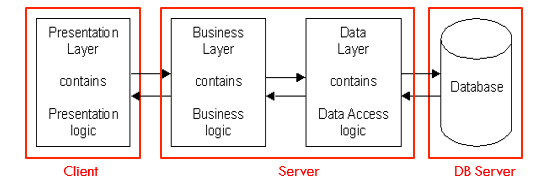
\includegraphics[scale=1]{Capture2.png} 
\begin{itemize}
\item A Presentation Layer that sends content to browsers in the form of HTML/JS/CSS. 
\item An Application Layer that uses an application server and processes the business logic for the application. This might be written in C\# or JavaScript.
\item A Data Layer which is a database management system that provides access to application data. This could be SQL Server or Azure. \\
\end{itemize}
\subsubsection{Benefits}
\begin{itemize}
\item It gives you the ability to update the technology stack of one tier, without impacting other areas of the application.
It allows for team members to each work on their own areas of expertise.
\item You are able to scale the application up and out. A separate back-end tier, for example, allows you to deploy to a variety of databases instead of being locked into one particular technology. It also allows you to scale up by adding multiple web servers.
\item It adds reliability and more independence of the underlying servers or services.
\item It provides an ease of maintenance of the code base, managing presentation code and business logic separately, so that a change to business logic, for example, does not impact the presentation layer. \cite{tier}
\end{itemize}
\subsection{Front-end Interface Method}
A web application which allows for browser support will be created. There it should work on most browsers including mobile browsers.
\subsection{Back-End Service}
ASP.net MVC uses SQL Server and we will use a cloud service such as Azure or Amazon web services.
\subsection{Other Supporting Software}
Dot Net Highcharts will be used for any reporting functionality we might have.Bootstrap will also be used to make sure that the web app looks good and works on all browsers. \\
\subsection{Student Responsibilities}
\begin{itemize}
\item Abdulkadir Dere - Group Leader
\item Brenda Lin - Quality Assurance
\item Jesse Wright - Technical Lead
\item Liam Leibrandt - Analysis Lead
\end{itemize}
\subsection{Sprint Plan}
\subsection{Use Case Diagram}
\subsection{Class Model Diagram}
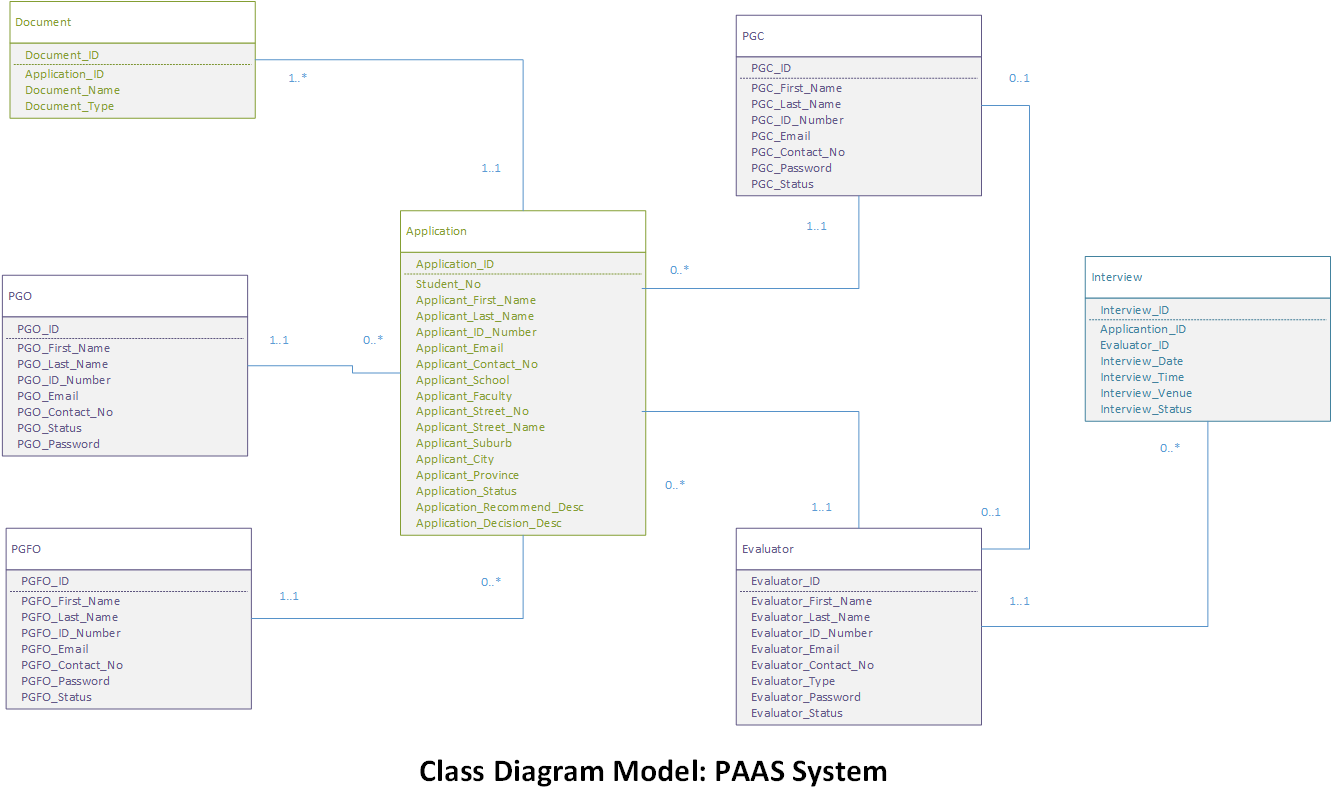
\includegraphics[scale=0.5]{ERD.png} \\
\subsection{Process Model(Flow Models)}
\subsection{Sequence Diagrams}
\subsection{State Machine Diagrams}

\section{Implementation (User Manual)}

\section{Testing}
\subsection{Functionality Testing}
\subsubsection{Motivation for Functionality Testing} 
Functionality testing is very important because it allows us to check and ensure that all functions that we have implemented for our system’s use
cases, are running correctly. This ensures that the data passed from users through the functions (via field forms) to the database is accurate and
without errors. This also allows us to determine if any use cases/processes contain faulty logic or flow so that we may review and alter them. 
\subsubsection{Case Name: Create a New Application} 
\begin{tabu} to \textwidth {| X[l] | X[l] | X[l] | X[l] | X[l] | X[l] | X[l]|}
\hline
\textbf{Test Number} & \textbf{Action/ Test} & \textbf{Test Input} & \textbf{Expected Results} & \textbf{Actual Results} & \textbf{Pass/Fail} & \textbf{Comments} \\
\hline
\end{tabu}
\subsection{Interface Testing}
\subsubsection{Motivation for Interface Testing} 
Interface testing is very important because this is the view that our end-user interacts with in order to use the functionality of our system. We have to ensure that the interface features, components and tools run correctly. We have to ensure that the user is never confused as to how to use our system and its functions. If our interface is not user-friendly then it is highly unlikely that anyone would make use of our web-
application.
\subsection{Security Testing}
\subsection{Cross-Browser Compatibility Testing}
\subsubsection{Motivation for Cross-Browser Compatibility Testing} 
Cross browser testing is the process of testing a web application across different browsers to ensure that a web application works as intended across multiple browsers since certain components might work differently on different web browsers. \\ \\
We shall test our web application on the following web browsers: \\ 
\begin{itemize}
\item Microsoft Edge version 40.15063.0.0
\item Google Chrome version 60.0.3112.113
\item Mozilla Firefox version 55.0.3 
\end{itemize}
Desktop Browser tests have been conducted on Windows 10 operating system. \\ \\
Mobile Browser tests have been conducted on Android 7.0 Nougat operating system. 
\subsubsection{Test Case Name: Check Cross-Browser Compatibility}
Requirement Description: The system should be compatible with different types of browsers \\ \\
\begin{tabu} to \textwidth {| X[l] | X[l] | X[l] | X[l] | X[l] | X[l] | X[l]|}
\hline
\textbf{Test Number} & \textbf{Action/ Test} & \textbf{Test Input} & \textbf{Expected Results} & \textbf{Actual Results} & \textbf{Pass/Fail} & \textbf{Comments} \\
\hline
1. & Access the Web Application using the Google Chrome Desktop browser (version 60.0.3112. 113) & Run the PAAS Web Application on Google Chrome Desktop Browser (version 60.0.3112. 113) &  The user should be able to view and interact with the PAAS website, including login into the system & The system did as expected & Pass & \\
\hline
2. & Access the Web Application using the Google Chrome Mobile browser (version 60.0.3112. 116) & Run the PAAS Web Application on Google Chrome Mobile Browser (version 60.0.3112. 116) &  The user should be able to view and interact with the PAAS website, including login into the system & The system did as expected & Pass & \\
\hline
3. & Access the Web Application using the Mozilla Firefox Desktop browser (version 55.0.3) & Run the PAAS Web Application on Mozilla Firefox Desktop Browser (version 55.0.3) & The user should be able to view and interact with the PAAS website, including login into the system & The system did as expected & Pass & \\
\hline
4. & Access the Web Application using the Mozilla Firefox Mobile browser (version 55.0.2) & Run the PAAS Web Application on Mozilla Firefox Mobile Browser (version 55.0.2) & The user should be able to view and interact with the PAAS website, including login into the system & The system did as expected & Pass & \\
\hline
5. & Access the Web Application using the Microsoft Edge browser (version 40.15063.0.0) & Run the PAAS Web Application on Microsoft Edge browser (version 40.15063.0.0) & The user should be able to view and interact with PAAS website, including login into the system & The system did as expected & Pass & \\
\hline
\end{tabu}
\subsection{Test Summary}
Cross Browser Compatibility Test was successful for all the specified browsers except Microsoft Edge. Microsoft Edge does not display the Date Picker. So, the user cannot view Date Picker hence they can’t select a date. This feature works well with other browsers. After analyses and research, we have found that Microsoft Edge has default style and selector for date. The default style takes precedence over additional styling done through the plugin. The user can still enter a date manually with the format of “yyyy/mm/dd”. This is problematic as the does not know the format hence will not be able to enter the correct date format. This issue is noted and will be fixed in construction phase.

\begin{thebibliography}{9}
\bibitem{product-design}
Clark Wimberly, sitepoint \\
\texttt{https://www.sitepoint.com/5-simple-ux-principles-guide-product-design/}

\bibitem{Scrum}
Scrum Alliance, \\
\texttt{https://www.scrumalliance.org/why-scrum}

\bibitem{tier}
Bob Pepalis, IZENDA, \\
\texttt{https://www.izenda.com/blog/5-benefits-3-tier-architecture/}

\end{thebibliography}

\end{document}
